%########################################
%CS 461 CAPSTONE 
%GROUP 20 - Griffin Gonsalves, Paul Kwak, Shawn Cross
%FALL 2016
%########################################
\documentclass[letterpaper, 10pt, draftclsnofoot, compsoc, onecolumn]{IEEEtran}
\usepackage[latin1]{inputenc}
\usepackage[T1]{fontenc}
\usepackage[english]{babel}
\usepackage{amsmath}
\usepackage{amssymb,amsfonts,textcomp}
\usepackage{color}
\usepackage{array}
\usepackage{supertabular}
\usepackage{hhline}

\usepackage{hyperref}
%\usepackage{digsig} %not a default package... just for signature field on final page.
\usepackage{comment}

\hypersetup{pdftex, colorlinks=true, linkcolor=black, citecolor=blue, filecolor=blue, urlcolor=blue, pdftitle=SYSTEMS AND SOFTWARE REQUIREMENTS SPECIFICATION (SSRS) TEMPLATE, pdfauthor=Clinton Jeffery, pdfsubject=, pdfkeywords=}
\usepackage[pdftex]{graphicx}
% Outline numbering
\setcounter{secnumdepth}{3}
\renewcommand\thesection{\arabic{section}}
\renewcommand\thesubsection{\arabic{section}.\arabic{subsection}}
\renewcommand\thesubsubsection{\arabic{section}.\arabic{subsection}.\arabic{subsubsection}}

\parskip 1.5ex plus 0.2ex minus 0.1ex
\makeatletter

\newcommand\arraybslash{\let\\\@arraycr}
\makeatother
% Page layout (geometry)
\setlength\voffset{-1in}
\setlength\hoffset{-1in}
\setlength\topmargin{0.5in}
\setlength\oddsidemargin{.75in}
\setlength\evensidemargin{.75in}
\setlength\textheight{8.278in}
\setlength\textwidth{6.5in}
\setlength\footskip{0.561in}
\setlength\headheight{0.5in}
\setlength\headsep{0.461in}
% Footnote rule
\setlength{\skip\footins}{0.0469in}
\renewcommand\footnoterule{\vspace*{-0.0071in}\setlength\leftskip{0pt}\setlength\rightskip{0pt plus 1fil}\noindent\textcolor{black}{\rule{0.25\columnwidth}{0.0071in}}\vspace*{0.0398in}}
% Pages styles
\makeatletter
\newcommand\ps@Standard{
  \renewcommand\@oddhead{\hfill }
  \renewcommand\@evenhead{\@oddhead}
  \renewcommand\@oddfoot{\foreignlanguage{english}{\textcolor{black}{SSRS Page }}\foreignlanguage{english}{\textcolor{black}{\thepage{}}}}
  \renewcommand\@evenfoot{\@oddfoot}
  \renewcommand\thepage{\arabic{page}}
}
\newcommand\ps@FirstPage{
  \renewcommand\@oddhead{}
  \renewcommand\@evenhead{\@oddhead}
  \renewcommand\@oddfoot{}
  \renewcommand\@evenfoot{\@oddfoot}
  \renewcommand\thepage{\arabic{page}}
}
\makeatother
\pagestyle{Standard}
%\setlength\tabcolsep{1mm}
\renewcommand\arraystretch{1.3}
% footnotes configuration
\makeatletter
\renewcommand\thefootnote{\arabic{footnote}}
\makeatother
\title{Forge VR Explorer Requirements}
\author{Shawn Cross, Griffin Gonsalves, Paul Kwak}
\date{2016-11-3}


%\usepackage{etoolbox}
%\patchcmd{\thebibliography}{\section*{\refname}}{}{}{}
\begin{document}

\clearpage\setcounter{page}{1}\pagestyle{Standard}
\thispagestyle{FirstPage}

\bigskip

{\centering\selectlanguage{english}\bfseries\color{black}
Forge VR Explorer Requirements
\par}


\bigskip

{\centering\selectlanguage{english}\bfseries\color{black}
November 4 2016
\par}
\bigskip
\bigskip
\bigskip
\bigskip
\bigskip
\bigskip
\bigskip
\bigskip
\bigskip
\bigskip
\bigskip
\bigskip
\begin{center}
	
\includegraphics[scale=0.8]{forge_logo.png}
\end{center}


\vfill
{\centering\selectlanguage{english}\bfseries\color{black}
Abstract
\par}

{\centering\selectlanguage{english}\mdseries\color{black}
	The Forge VR Explorer branches from an Autodesk prototype project called Vrok-It, which is a simple web-based 3D 
	model viewer and mobile virtual reality (VR) explorer. The project will expand upon its ability to display uploaded 3D 
	models in browser and in VR, and improve its accessibility. Conventionally, viewing 3D models in VR is a challenge if 
	you have model files on many devices, or have a headset that only works in conjunction with a smartphone. The 
	Forge VR Explorer aims to do this by utilizing a web-based software that uses the features of the Autodesk Forge API. 
	The project will also be expanded with new ideas and stretch goals as the project is developed.
\par}

\bigskip
\bigskip

\clearpage{\centering\selectlanguage{english}\bfseries\color{black}
SYSTEMS AND SOFTWARE \ REQUIREMENTS SPECIFICATION (SSRS) FOR 
\par}

\bigskip

{\centering\selectlanguage{english}\bfseries\color{black}
Forge VR Explorer
\par}

\bigskip
\bigskip
\bigskip

\begin{figure}
\centering
%\includegraphics[width=3.4362in,height=0.6134in]{SSRSTemplateA2-img1.png}
\end{figure}

\bigskip
\bigskip

{\centering\selectlanguage{english}\bfseries\color{black}
Version 1.0
\par}

{\centering\selectlanguage{english}\bfseries\color{black}
11/4/2016
\par}


\bigskip
\bigskip

{\centering\selectlanguage{english}\bfseries\color{black}
Prepared for:
\par}

{\centering\selectlanguage{english}\bfseries\color{black}
Patti Vrobel, Autodesk
\par}


\bigskip
\bigskip

{\centering\selectlanguage{english}\bfseries\color{black}
Prepared by:  
\par}

{\centering\selectlanguage{english}\bfseries\color{black}
Shawn Cross, Griffin Gonsalves, Paul Kwak
\par}

{\centering\selectlanguage{english}\bfseries\color{black}
Oregon State University
\par}

{\centering\selectlanguage{english}\bfseries\color{black}
Corvallis, OR \ 97331
\par}

\clearpage{\centering\selectlanguage{english}\bfseries\color{black}
\foreignlanguage{english}{\MakeUppercase{\ }}\foreignlanguage{english}{\MakeUppercase{Forge VR Explorer SSRS}}
\par}

{\centering\selectlanguage{english}\bfseries\color{black}
TABLE OF CONTENTS
\par}

\bigskip

{\selectlanguage{english}\bfseries\color{black}
Section\ \ Page}

\setcounter{tocdepth}{9}
\renewcommand\contentsname{}
\tableofcontents

\bigskip
\clearpage

\section{Introduction}
	The system being developed is intended to be a place in which users with CAD files can go and easily view and explore those files in both a 3D viewer and optionally in VR. The user will also be able to move through the models depending on the model that they are currently viewing. This provides a solution to those who don't have access to an expensive CAD program or VR headset as it will be a free to use web application that is usable with inexpensive VR equipment such as Google cardboard. This app is aimed at people that would want to explore a 3D model without any experience with VR or a CAD program.
 

\subsection{Scope}
	The scope of this project includes developing a new website hosting a web application.
 	This software should allow for the upload of a 3D model file to be viewed in browser as well as in a VR environment. 
	This project also aims to reduce barriers from uploading and viewing files by implementing different Forge APIs in order to improve the users 
	overall experience while using the website.

\subsection{DEFINITIONS, ACRONYMS, AND ABBREVIATIONS}
	\begin{description}
	\item{CAD} Computer Aided design is software used to design and view 3D models.

	\item{CAD file} The type of files that can be uploaded to the website for viewing in the Forge viewer. 
	We will  narrow down what types of files can be used as we progress through the development process.

	\item{FORGE}~\cite{forge2016} A collection of API services provided by Autodesk that provide 3D modeling services and tools.

	\item{Forge Viewer} This is one of the APIs in Forge. It displays 3D models from CAD files and also allows
	for user interaction.
	
	\item{Model Derivative API} This is another API in Forge. It can generate SVF files that we can utilize in the application from other model filetypes.
	
	\item{VR} Acronym for virtual reality, typically a peripheral device or smartphone
	\item{exploding model} A model viewing functionality that separates components from their original locations in order to gain an alternate view of the model.
	\end{description} 

\clearpage
	
%\subsection{REFERENCES}
\bibliography{bibfile}
\bibliographystyle{IEEETran}

\clearpage

\section{OVERALL DESCRIPTION}

\subsection{PRODUCT PERSPECTIVE}
	The product would be jump-started from the Vrok-It~\cite{Vrok-It2016} platform that has already been created. 
	We are to create a new site with some of these assets in order to provide a new experience focused on exploring a model in 3D. 

\subsection{PRODUCT FUNCTIONS}
	\begin{enumerate}
	 	\item The user is able to choose a CAD model file locally or upload one from another cloud service.
	 	
		\item Once a model is chosen or a file is uploaded the 3D models will be seen in the Forge viewer at the center of the website.
		
		\item The user will have the ability to connect a smartphone device to the website through the use of a QR scanner.

		\item Once the user has connected their a smartphone the model should be able to be viewed in VR with a the use of a VR headset such as Google Cardboard, if supported. 
		
		\item "Viewable" 3D models can be interacted with by the user in the Forge viewer in several different ways.		
		
		\item The user will be able to manipulate the model and observe in VR.
	\end{enumerate}

\subsection{USER CHARACTERISTICS}
	%perhaps easier if itemized
	When finished this product should be usable by anyone that has access to a CAD model file. If the user is wanting to use the VR 
	portion of the website then they will need access to some sort of VR headset. If the user does have access to a VR headset they 
	should not need any extra knowledge other than how to use the headset.  

\subsection{SYSTEM LEVEL (NON-FUNCTIONAL) REQUIREMENTS}

\subsubsection{Software Interfaces}
	\begin{itemize}
		\item Interface between the computer and the website, for the uploading of models from a user's local machine into the 
		website for viewing. 
	
		\item Input will be any 3D model which is sent to the model derivative api to be converted to SVF, then to the Forge Viewer where it is displayed.
	
		\item Interface between the website and the device the user wishes to view the model on. Currently vrok.it uses a QR code to accomplish this-Input is the QR code scanned by the phone, output is the manipulatable model in an environment 
	for viewing. 
	\end{itemize}
	

\subsubsection{User Interfaces}

	\begin{itemize}
		\item The main user interface will be the web application in which the user will be able to upload a  model and then view it in the Forge viewer on the  webpage. 
		\item The user will be able interact and manipulate the model inside the viewer using an interface. This interface can rotate, move, show an exploded view of the model, and more.
		\item On a smartphone, the webpage loads a compact version of the main site. 
		\item The viewer on the smartphone is fullscreen when connected, and will be manipulated the same way the webpage is currently manipulating the model.
		\item The user will be able to navigate through the model in VR using a VR headset.
	\end{itemize}

\section{SPECIFIC REQUIREMENTS}
\bigskip

\subsection{SYSTEM FEATURES}
\medskip

\subsubsection{File Uploading}

\begin{enumerate}
	\item This will allow the user to be able to upload any models that they have access to the website.

	\item
	\begin{description} 
		\item[Input] The user will select a file from their computer that they would like to upload to the website. 
		\item[Output] Finishing the upload process the model that was in the file should now be viewable on the website. 
	\end{description}

	\item
	\begin{enumerate}
		\item The user should be able to upload his/her file to the website using a standard pop-up window.
		\item The software must determine if the file is a reasonable size(<50MB), and is an accepted format. 
		\item After the file is uploaded, it is then made available to the other components of the software to be used.
		\item Users should be notified if their file was unable to be uploaded.
		\item The uploaded file should be displayed in the list of usable models on the webpage.
	\end{enumerate}
\end{enumerate}
%end of upload feature

\subsubsection{Viewable Model}

\begin{enumerate}
	\item	The user should be able to see the model that they have chosen or uploaded to the site in the Forge viewer. They 
	should also be able to interact with that model in the Forge viewer. 

	\item
	\begin{description}
		\item[Input] The user will chose from the list of predefined models or upload their own model. 
		\item[Output] The model will now be view able in the large model viewer and the user should be able to interact with that model.
	\end{description}

	\item The model must not be so large or detailed that the website can not render it.

	\item The model should be displayed in full in the Forge viewer and should not be hard to interact with. 

	\begin{enumerate}
		\item The viewer will be displayed at the center of the wepage.
		\item Once the user has selected a model for viewing or uploaded their own model, it will be displayed in the viewer. 
		\item This window must be interactive, and display the user's model correctly.
		\item The viewer should be able to display a reasonably sized(<50MB) model. 
	\end{enumerate}
\end{enumerate}
%end of feature 2

\subsubsection{Smartphone Connection}

\begin{enumerate}

	\item This will enable the users to connect their phone to the Vrok-It website. This is needed so that the user will be able to view their model in a VR environment through the use of their phone and a compatible VR headset. 

	\item
	\begin{description}
		\item[Input] The user will scan a QR code located on the main page of website with a QR scanning application on their phone. 
		\item[Output] The model that is currently loaded into the Forge viewer on the website will now be displayed on the phone and ready to
		be viewed in VR. 
	\end{description}

	\item The user must have a device that is capable of using a QR scanning application. The phone also has access to an Internet 
	connection to be able to connect to the websites current session. 
	
	If the user opts to view the model in VR, then a VR headset is also required for the user's device.

	\item The phone should be connected to the website within a few seconds. This might vary depending on how good of an Internet 
	connection the user currently has. 

	\item
	\begin{enumerate}
		\item In order to provide VR functionality for an android device, the software must first establish a connection. 
		\item Using a QR scanner, the android device will be linked to a mobile version of the viewer displayed in stereoscopic format. 
		\item This requires a stable Internet connection in order to deliver the content to the device.
	\end{enumerate}
\end{enumerate}
%end feature 3

\subsubsection{Forge Authentication}
\begin{enumerate}
	\item This is used to get authentication and authorization when using Forges other APIs. This provides security for the users using 
	the APIs on the website. 

	\item The token will be created automatically every time a user accesses the website.

	\item The user must be able to gain access to the website on a laptop or desktop.

	\item 
	\begin{enumerate}
		\item During the loading of the web page the authentication API should generate a token For the user in case they want to use 
		either the data management API or the model derivative API. 
	\end{enumerate}
\end{enumerate}
%end of feature 4

\subsubsection{Data Management}

\begin{enumerate}
	\item Users that have files in A360 or in Fusion 360 should be able to gain access through those files from the
	website.

	\item
	\begin{description} 
		\item[Input] The user should be able to identify that they want to gain access to their files on either A360/Fusion360 or local. 
		\item[Output] Using the Forge Data Management API the user should then have access to both of these Cloud storage sites to then upload a file.
	\end{description}

	\item
	\begin{itemize}
		\item The authentication API must have created a Token for the API to use.
		\item Must have an account with either A360 or Fusion 360. 
		\item Must conform to API general use cases
	\end{itemize}

	\item
	\begin{itemize}
		\item The files should load in a viewable format.
		\item The files should only be visible if they are viewable if not the user should be notified that the file
			they were trying to upload was unable to be used.
	\end{itemize}
	
	\item 
	\begin{enumerate}
		\item A place where users can enter information to gain access to their outside files. 
		\item This should be done through the use of the Forge Data Management API. 
		\item Once the user has access to these accounts they should then be able to obtain the 
		files they want to use and upload them to the Forge viewer.
	\end{enumerate}
\end{enumerate}
%End of feature 5

\subsubsection{Model Derivative}

\begin{enumerate}
	\item With the use of the Forge Model Derivative API any of the files that the user uploads will be converted into SVF files
	that are used by the model viewer
	
	\item
	\begin{description}
		\item[Input] The user will upload a CAD drawing file that they want to convert to an SVF file. 
		\item[Output] This should then return the correctly converted SVF file and it should now appear in the list of 
		viewable models on the website. If the conversion fails the user should be notified of the failure.
	\end{description}

	\item
	\begin{itemize}
		\item The authentication API must have created a Token for the model derivative API to use.
		\item The user must have used the proper CAD files to be converted. 
	\end{itemize}

	\item The program should clearly display the model in the list of viewable models.

	\item
	\begin{enumerate}
		\item The website will take the files that have been uploaded by the user and convert them to the appropriate file
		format.
		\item The website should notify the user if the file conversion has failed.
	\end{enumerate}   
\end{enumerate}
%End of feature 6

\begin{comment}
\subsubsection{Hardware Detection}

\begin{enumerate}
	\item This feature serves as a way for the software to understand the hardware its being run on. This will be the foundation for 
	giving a user feedback on potential experience viewing.

	\item
	\begin{description}
		\item[Input] The user connects their phone to Vrok-It through the use of a QR scanner. 
		\item[Output] After connection it should verify what type of device that the user has connected.
	\end{description}

	\item	Reliance on the user giving permission to allow the software to get information about hardware specifications. Similar to 
	Androids permissions the user many not want to give information out so our hardware detection may be hindered and 
	unable to function at all. 

	\item Needs to be able to obtain hardware specification as fast as possible to give users feedback immediately. The sooner 
	our software understands the user's hardware the faster it can give a recommendation about optimal viewing. 

	\begin{enumerate}
		\item The software must be able to detect the user's smartphone when it connects using the QR code provided. 
		\item When a connection is made, the software will then detect the device, verify it is supported. 
		\item If device is known, the software then will use presets for the viewer on the device, otherwise
		it should alert the user about incompatibility and performance conflicts. 
		\item These alerts will inform the user that the device will not operate optimally with the project. 
	\end{enumerate}
\end{enumerate}
%end of feature 7
\end{comment}

\subsubsection{VR device support}

\begin{enumerate}
	\item View the model currently in the viewer in a VR environment using a VR headset such as Google cardboard. The user should also
	be able move through the model in VR. This could be extended to higher end VR devices later if time permits.

	\item
	\begin{description}
		\item[Input] A functioning model uploaded to the project site and displayed in the viewer.
		\item[Output] A model displayed on the user's device that is ready to be viewed with a VR headset.
	\end{description}

	\item Depends heavily on hardware on the device that the user is using. Devices with low-end hardware will likely not be able to 
	display models that are large or have a lot of detail very well.  

	\item The models need to be able to be manipulated by the viewer. If they are too large, the models will cause errors if they are 
	modified within the viewer.  

	\begin{enumerate}
		\item The VR model viewer displayed on the Android device must be supported on Google Cardboard's lenses. 
		\item The model must be tracked properly in the model viewer. 
		\item The model displayed on the users devices should mimic any interaction that happens to the model on the webpage.
		\item The user should have the ability to navigate through the model. 
	\end{enumerate} 
\end{enumerate}
%end of feature 8

\begin{comment}
\subsubsection{Website Redesign}

\begin{enumerate}
	\item In order to accommodate for new features, we would like to redesign the landing, and key interaction areas of the website using React. This will increase the site's usability by decreasing the amount of time used to interact with the website and making the site look more cohesive and presentable.
	\item This website must support the Forge API, the Forge viewer, and must be viewable on a smartphone browser. 
	\item The website must be able to properly load and display the project assets like the Forge Viewer. 
	\item The updated site will include a new main page for the project, as well as being able to expand the site as necessary.
	\item Key functionality such as uploading a model file and viewing the file should be clearly visible to the user.
		
\end{enumerate}
%end of feature 9
\end{comment}

\clearpage
\section[GANTT CHART/SIGNATURES]{\selectlanguage{english}\rmfamily\bfseries\color{black}
GANTT CHART \& SIGNATURES}

\begin{center}
	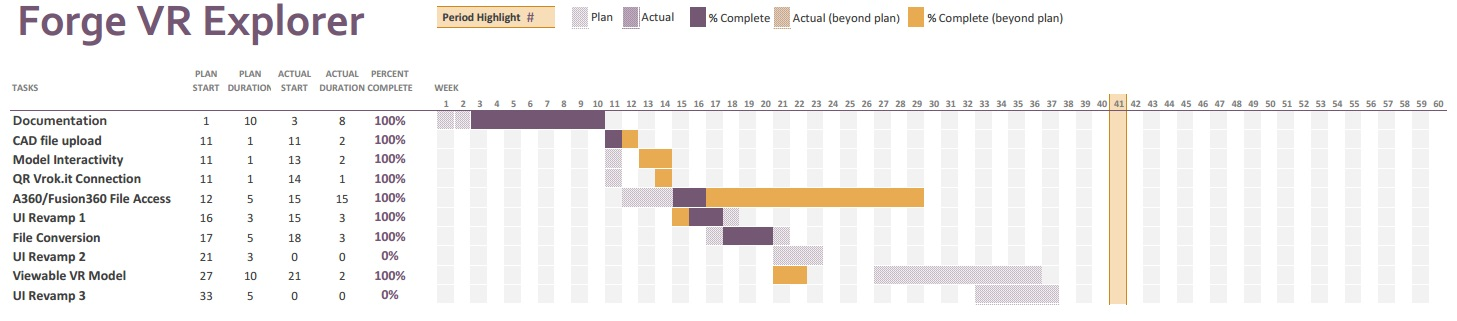
\includegraphics[scale=0.8]{GanttChart.jpg}
\end{center}

\newpage
\null
\vfill
%\clearpage\setcounter{page}{1}\pagestyle{Convertvi}
\begin{flushleft}


	\begin{Form}
		\rule{5in}{.4mm}\\
			Patti Vrobel\hspace{60ex}Date
	\end{Form}
		
	\vspace{1cm}	
	
	\rule{5in}{.4mm}\\
	Griffin Gonsalves\hspace{55ex}Date
		
	\vspace{1cm}	
	
	\rule{5in}{.4mm}\\
	Shawn Cross\hspace{59ex}Date
	
	\vspace{1cm}	
	
	\rule{5in}{.4mm}\\
	Paul Kwak\hspace{61ex}Date

\end{flushleft}

\end{document}
